\section{Master Module (MA)}

The MA module is composed of six modules:

\begin{enumerate}
    \item Display (DP): present process info to the user.
    \item Watchdog Timer (WD): supervise program flow of \mu M.
    \item Slave Switch (SS) : control power supply to Slave Module (SL).
    \item \mu C Master (\mu M): run the water flow measurement firmware.
    \item Bus Isolation (BI$_1$, BI$_2$): prevent back-powering via GPIO and I2C when SL is switched off.
    \item Opto Switch Driver (OD): control power supply to the Optical Sensor Module (OS).
\end{enumerate}


\begin{figure}[h]
    \centering
    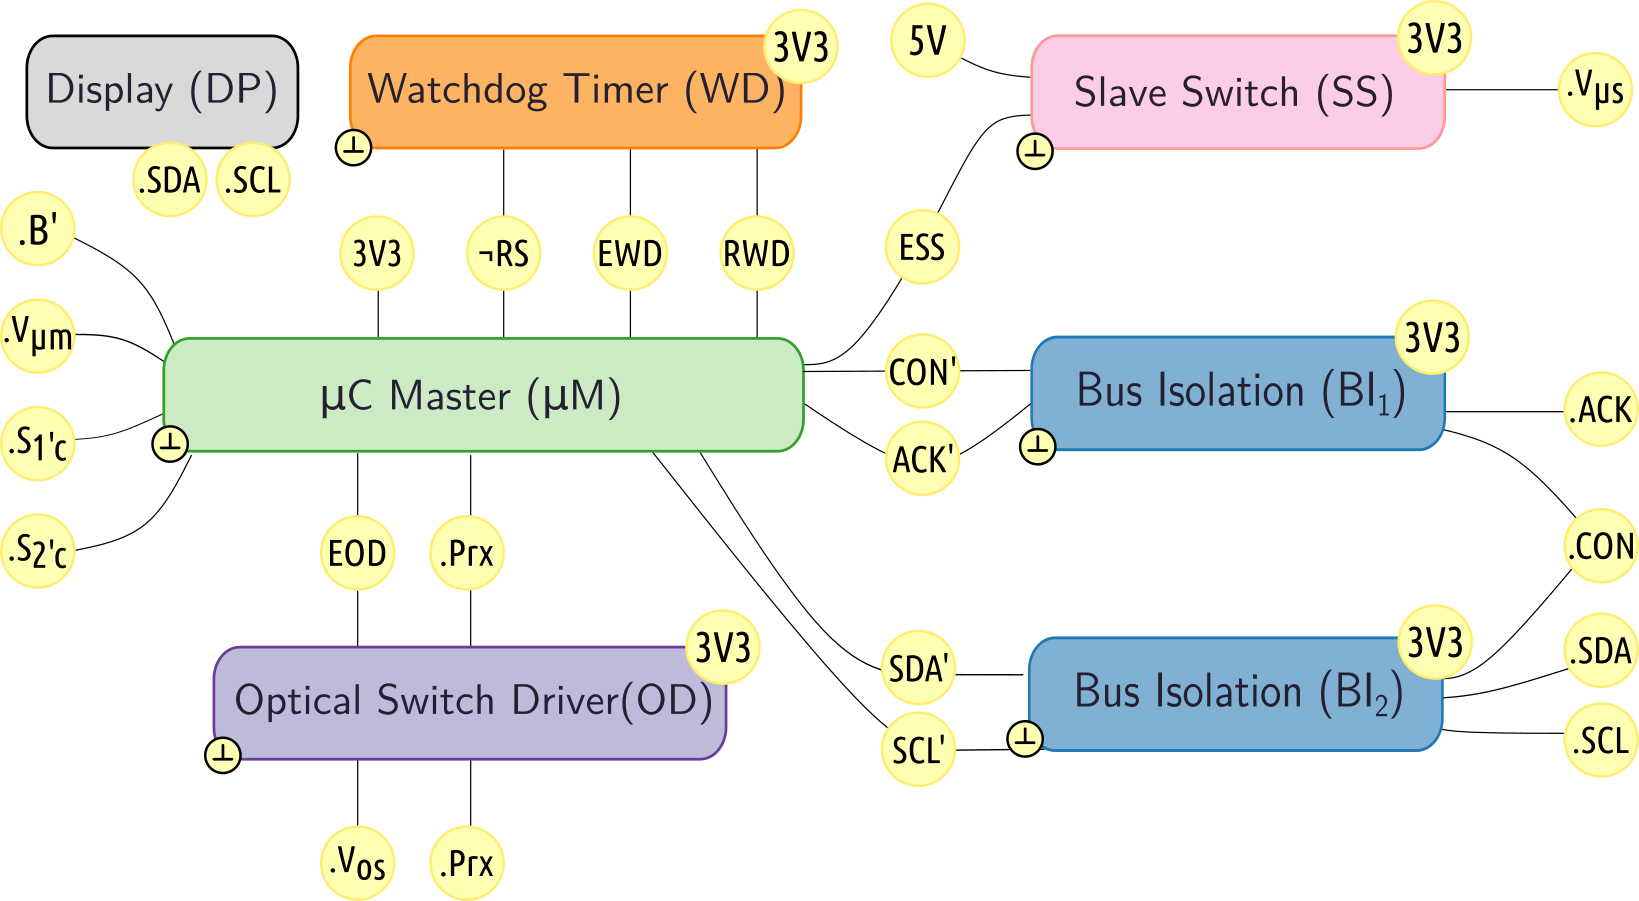
\includegraphics[width=1.0\textwidth]{MA/MA}
\end{figure}


\begin{table}[H]
    \centering
    \begin{threeparttable}[b]
        \begin{tabularx}{\linewidth}{ >{\hsize=0.15\hsize}X >
                    {\hsize=0.15\hsize}X > {\hsize=0.25\hsize}X >{\hsize=3.45\hsize}X}
            Id & Rank & Name             & Net description                                            \\
            \midrule
            1  & 1    & 3.3V             & voltage provided by \mu M                                  \\
            3  & 4    & \texttt{ESS}     & enable SS                                                  \\
            4  & 4    & \texttt{CON'}    & slave: are slave I2C bus and master I2C  connected ?       \\
            5  & 4    & \texttt{ACK'}    & slave: is slave  ready to receive I2C data from master   ? \\
            6  & 4    & \texttt{EOD}     & enable OD                                                  \\
            7  & 4    & \neg \texttt{RS} & watchdog timer reset due to a software or hardware defect  \\
            8  & 4    & \texttt{EWD}     & enable watchdog timer at the end of the startup code       \\
            9  & 4    & \texttt{RWD}     & reset ("kick") watchdog time to prevent a reset of $U_1$   \\
            10 & 4    & \texttt{SDA}     & master I2C data                                            \\
            11 & 4    & \texttt{SCL}     & master I2C clock                                           \\
        \end{tabularx}
        \begin{tablenotes}
            \item [-]
        \end{tablenotes}
    \end{threeparttable}
    \caption{MA - Netlist}
\end{table}

\subsection{Display Module (DP) }
\label{sec:DP}
The Display Module (DP) presents information on the ongoing metering process. This includes:

\begin{itemize}
    \item timestamp: current date and time
    \item process state: accumulating, transmitting, requesting internet time, ...
    \item power: battery voltage, solar panel voltage
    \item SD-Card reader: current filename
\end{itemize}

\subsubsection{Requirements}
We noticed the importance of providing comprehensive diagnostic information at the location of deployment.
The hardware is located inside a street gully which is exposed to humidity, dirt and mosquitos. When inspecting the system, the technician
must be able to diagnose a potential problem at a glance. He must be able to quickly decide if the unit must be dismounted and sent to the lab.
The display must therefore be clearly visible from every angle. This excludes LCD displays.
Given the absence of grid-connection, low power consumption is mandatory. This excludes LED displays.

\subsubsection{Implementation}
We use a small,
inexpensive OLED with very low power consumption of only \qty{30}{\nA}.
\begin{figure}[h]
    \centering
    \includegraphics[width=0.2\textwidth]{MA/DP/DP}

\end{figure}


\begin{table}[H]
    \centering
    \begin{threeparttable}[b]
        \begin{tabularx}{\linewidth}{ >
                    {\hsize=.25\hsize}X >
                    {\hsize=0.5\hsize}X >
                    {\hsize=.25\hsize}X  >
                    {\hsize=.5\hsize}X >
                    {\hsize=.25\hsize}X  >
                    {\hsize=3\hsize}X
            }
                  & \multicolumn{4}{c}{Pin mapping} &                                                    \\
            \cmidrule(lr){3-6}
            Id    & Net                             & Nb. & Name         & Type               & Function \\
            \midrule
            $U_1$ & .3V3                            & 4   & \texttt{VCC} & \rightharpoonup    &          \\
            $U_1$ & .GND                            & 5   & \texttt{GND} & \rightharpoonup    &          \\
            $U_1$ & .SCL                            & 6   & \texttt{SCL} & \leftharpoonup     &          \\
            $U_1$ & .SDA                            & 7   & \texttt{SDA} & \leftrightharpoons &          \\
        \end{tabularx}
    \end{threeparttable}
\end{table}


\begin{table}[H]
    \centering
    \begin{tabularx}{\linewidth}{>{\hsize=0.25\hsize}X
            >{\hsize=1\hsize}X >{\hsize=1\hsize}X
            >{\hsize=0.5\hsize}X >{\hsize=2.25\hsize}X}
        Id    & BOM Item                 & Order Code  & Package & Rationale     \\
        \midrule
        $U_1$ & \cite{noauthor_096_2021} & WPI438 / 59 & DIL (4) & I2C interface \\
    \end{tabularx}


\end{table}
\clearpage
\subsection{Watchdog Module (WD) }
\label{sec:WD}

The Watchdog Module (WD) module prevents unexpected or intermittent software or hardware failures from stalling the microcontroller
indefinitely. The module expects a timer reset signal from the microcontroller withing a given period. In the absence of this
event, the watchdog circuit will reset the \mu C.

\subsubsection{Requirements}

The application runs only every second or so and the \mu C is
in power-saving mode most of the time. There are no strict timing requirements but unnecessary watchdog resets must be avoided.
This means that the watchdog circuit must be configurable for timeout periods of several seconds.
This requirement excludes many available watchdog ICs. \par

\begin{enumerate}
    \item supply voltage  \SI{3.3}{\V}.
    \item low power, low quiescent current.
    \item timeout period of several seconds.
\end{enumerate}

For my application, I choose a timeout period of roughly \SI{8}{\s}. This prevents any possible false resets due to
variations in program execution time that might be introduced by future software updates.

\subsubsection{Implementation}


\begin{table}[H]
    \centering
    \begin{threeparttable}[b]
        \begin{tabularx}{\linewidth}{
                >{\hsize=0.25\hsize}X
                >{\hsize=0.75\hsize}X
                >{\hsize=1.25\hsize}X
                >{\hsize=0.5\hsize}X
                >{\hsize=2.25\hsize}X
            }
            Id    & Desc                         & Order Code       & Package & Rationale                                         \\
            \midrule
            $U_1$ & \cite{noauthor_tps3431_2018} & TPS3431SDRBR/681 & VSON-8  & wide range of timeout values\tnote{1}             \\
            $R_p$ & 100k                         & generic          & 0603    & pull-up resistor\tnote{2}                         \\
            $C_c$ & \SI{100}{\nF}, \SI{16}{\V}   & generic          & 0603    & value for \approx \SI{8}{\s} timeout\tnote{3}     \\
            $C_b$ & \SI{100}{\nF}, \SI{16}{\V}   & generic          & 0402    & bypass cap, optional but recommended in datasheet \\
        \end{tabularx}
        \begin{tablenotes}
            \item [1] and low quiescent current, active-low open drain output suitable for Arduino dev board.
            \item [2] see \cite{noauthor_tps3431_2018}, 8.2.2.1 Calculating WDO Pullup Resistor Design 1.
            \item [3] see \cite{noauthor_tps3431_2018}, table 8-3.
        \end{tablenotes}
    \end{threeparttable}[b]
    \caption{WD Module - BOM}
    \label{table:wd1}
\end{table}

\begin{table}[H]
    \centering
    \begin{threeparttable}[b]
        \begin{tabularx}{\linewidth}{ >{\hsize=.15\hsize}X >{\hsize=1.35\hsize}X >{\hsize=1.5\hsize}X }
            \toprule
            Id & Issue                           & Potential solutions      \\
            \midrule
            1  & Make watchdog reset  persistent & add a flip-flop\tnote{1} \\
            \bottomrule
        \end{tabularx}
        \begin{tablenotes}
            \item [1] the state of the flip-flop could then be transmitted to alert a human supervisor that the circuit has malfunctioned.
        \end{tablenotes}
    \end{threeparttable}
    \caption{WD - issues}
\end{table}
\clearpage
\begin{figure}[h]
    \centering
    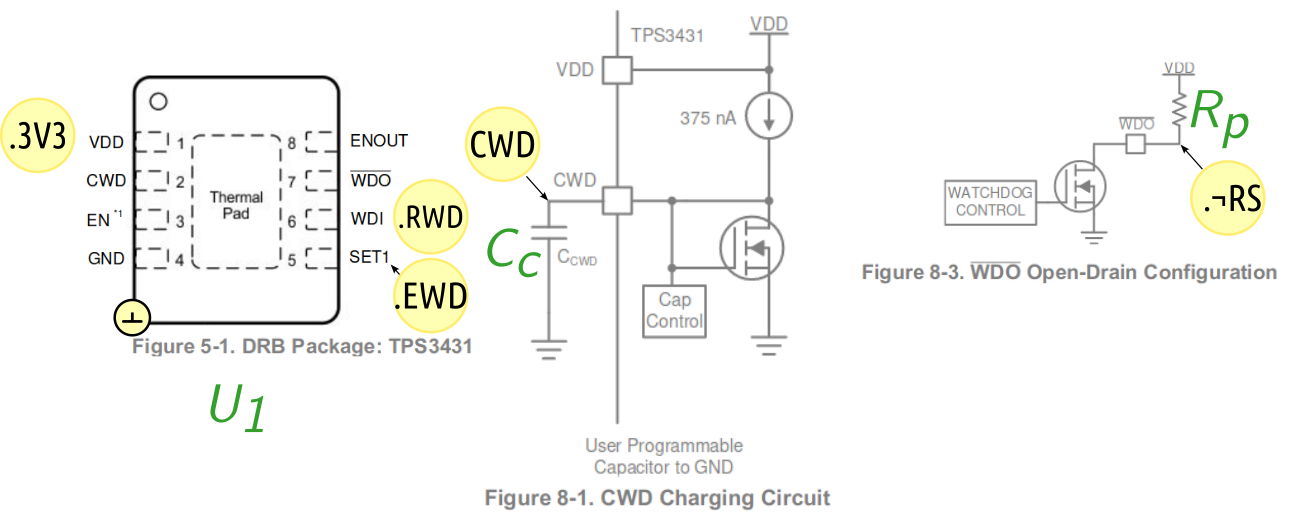
\includegraphics[width=1.0\textwidth]{MA/WD/WD}
    \caption{WD - schematic, from datasheet \cite{noauthor_tps3431_2018}}
\end{figure}

\begin{table}[H]
    \centering
    \begin{threeparttable}[b]
        \begin{tabularx}{\linewidth}{ >
                    {\hsize=.25\hsize}X >
                    {\hsize=0.5\hsize}X >
                    {\hsize=.25\hsize}X  >
                    {\hsize=.5\hsize}X >
                    {\hsize=.25\hsize}X  >
                    {\hsize=3\hsize}X
            }
                  & \multicolumn{4}{c}{pin} &                                                                                                   \\
            \cmidrule(lr){3-6}
            Id    & Net                     & Nb. & Name                        & Type            & Function                                    \\
            \midrule
            $U_1$ & .3V3                    & 1   & \texttt{VDD}                & $\leftarrow$    & power supply                                \\
            $U_1$ & CWD                     & 2   & \texttt{CWD}                & \leftsquigarrow & The timeout period is configured with $C_c$ \\
            $U_1$ & \Gnd                    & 4   & \texttt{GND}                & \Gnd            &                                             \\
            $U_1$ & .EWD                    & 5   & \texttt{SET1}               & \leftharpoonup  & enable timer                                \\
            $U_1$ & .RWD                    & 6   & \texttt{WDI}                & \leftharpoonup  & reset timer\tnote{1}                        \\
            $U_1$ & .\neg RS                & 7   & \texttt{\textoverline{WDO}} & \rightharpoonup & pin pulled down if timer expired            \\
            $U_1$ &                         & 3,8 & \texttt{EN}, \texttt{ENOUT} &                 & can be left floating for this application   \\
            $C_c$ & CWD                     & 1   & \texttt{1}                  &                 &                                             \\
            $C_c$ & \Gnd                    & 2   & \texttt{2}                  & \Gnd            &                                             \\
            $R_p$ & .\neg RS                & 1   & \texttt{1}                  &                 & open drain pullup                           \\
            $R_p$ & \Gnd                    & 2   & \texttt{2}                  & \Gnd            &                                             \\
            \bottomrule
        \end{tabularx}
        \begin{tablenotes}
            \item [1] pulled down by \mu M in regular intervals < 8 s during normal operation.
        \end{tablenotes}
    \end{threeparttable}
    \caption{WD - Pin mapping}
\end{table}


\clearpage




\subsection{Slave Switch Module (SS)}
\label{sec:SS}


The Slave Switch Module (SS) controls the power supply to the Slave Module (SL).
As explained previously in section \ref{sec:Too}, the slave is powered only during transmission in order
to reduce energy consumption mainly due to the relatively high standby current of the radio module.

\subsubsection*{Requirements}


The load switch must be able to switch the maximum current for both master and slave.
The maximum current is determined by the GMS module on the slave.
We expect the maximum to not exceed \SI{1}{\A}.

\subsubsection*{Implementation}


\begin{figure}[h]
    \centering
    \includegraphics[width=0.3\textwidth]{MA/SS/SS}
    \caption{SS - schematic, based on datasheet \cite{noauthor_tps22810_2016}}
\end{figure}

\begin{table}[H]
    \centering
    \begin{threeparttable}[b]
        \begin{tabularx}{\linewidth}{ >
                    {\hsize=.25\hsize}X >
                    {\hsize=0.5\hsize}X >
                    {\hsize=.25\hsize}X  >
                    {\hsize=.5\hsize}X >
                    {\hsize=.25\hsize}X  >
                    {\hsize=3\hsize}X
            }
                  & \multicolumn{4}{c}{Pin mapping} &                                                                   \\
            \cmidrule(lr){3-6}
            Id    & Net                             & Nb. & Name             & Type            & Function               \\
            \midrule
            $U_1$ & .5V                             & 1   & VIN              & \leftharpoonup  & input                  \\
            $U_1$ & \Gnd                            & 2   & \texttt{GND}     & \Gnd            &                        \\
            $U_1$ & .ESL                            & 3   & \texttt{EN/UVLO} & \rightharpoonup & switch enable          \\
            $U_1$ &                                 & 4   & \texttt{CT}      &                 & left floating\tnote{1} \\
            $U_1$ &                                 & 5   & \texttt{QOD}     &                 & left floating\tnote{2} \\
            $U_1$ & .V\textsubscript{\mu S}         & 6   & \texttt{VOUT}    & \rightharpoonup & output                 \\
        \end{tabularx}
        \begin{tablenotes}
            \item [1]  the Arduino is not a high current load for this switch.
            \item [2] we don't care how fast the charge at the output decreases.
        \end{tablenotes}
    \end{threeparttable}

\end{table}
\input{hardware/modules/MA/SS/SS_issues}
\begin{table}[H]
    \centering
    \begin{threeparttable}[b]
        \begin{tabularx}{\linewidth}{ >
                    {\hsize=0.25\hsize}X >
                    {\hsize=0.75\hsize}X >
                    {\hsize=1.25\hsize}X >
                    {\hsize=0.5\hsize}X >
                    {\hsize=2.25\hsize}X
            }
            Id    & BOM Item                      & Order Code       & FF       & Rationale                                                                               \\
            \midrule
            $U_1$ & \cite{noauthor_tps22810_2016} & TPS22810DBVR/710 & SOT-23/6 & low $R_{ON}$\tnote{1}, input voltage range down to \SI{2.7}{\V}, low quiescent current. \\
        \end{tabularx}
        \begin{tablenotes}
            \item [1] The \cite{noauthor_arduino_2016-1} requires a \SI{5}{\V} power supply which is
            regulated to \SI{3.3}{\V} on the board.

            The Arduino board uses the \cite{noauthor_ap7115_2017} voltage regulator.
            According to the datasheet, the dropout voltage is
            \SI{200}{\mV}. Therefore, the voltage supplied to the Arduino $V_{\mu M}$ must be greater than \SI{3.5}{\V}.
        \end{tablenotes}
    \end{threeparttable}
    \caption{SS - BOM}
\end{table}











\subsection{\mu Master Module (\mu M)}

\mu M is a microcontroller that runs software to acquire, accumulate and request transmission of water flow measurements.

\subsubsection{Requirements}
Almost any microcontroller is able to accomplish this task.
Physical space is not critical, therefore we use a readily available low cost  Arduino Development Kit (DK)
DK, rather than designing a custom board. Given the absence of more specific requirements,
I choose the \cite{noauthor_arduino_2016-1} .

\subsubsection{Implementation}


\begin{table}[H]
    \centering
    \begin{tabularx}{\linewidth}{>{\hsize=0.25\hsize}X
            >{\hsize=1\hsize}X >{\hsize=1\hsize}X
            >{\hsize=0.5\hsize}X >{\hsize=2.25\hsize}X}
        Id    & BOM Item                       & Order Code & Package  & Rationale                 \\
        \midrule
        $U_1$ & \cite{noauthor_arduino_2016-1} &            & DIL (28) & availability, ease of use \\
    \end{tabularx}
    \caption{\mu M - BOM}

\end{table}
\begin{table}[H]
    \centering
    \begin{threeparttable}[b]
        \begin{tabularx}{\linewidth}{ >{\hsize=.15\hsize}X >{\hsize=1.35\hsize}X >{\hsize=1.5\hsize}X }
            Id & Issue                                                 & Potential solutions                                             \\
            \midrule
            1  & $U_1$ has relatively high power consumption.\tnote{1} & low power \mu C (MSP430FR2311IPW16) and custom charger circuit. \\
            2  & $U_1$ requires a stable 5 V power supply.\tnote{2}    & see issue 1                                                     \\
        \end{tabularx}
        \begin{tablenotes}
            \item [1]   This is due to the microcontroller itself (SAM D21) and to the peripheral components (battery charger).
            \item [2]   Given that a \SI{3.7}{\V} LiPo battery is used, this requires a boost conversion which in turn implies losses.
        \end{tablenotes}
    \end{threeparttable}
    \caption{\mu M - Issues}

\end{table}
\clearpage
\begin{figure}[h]
    \centering
    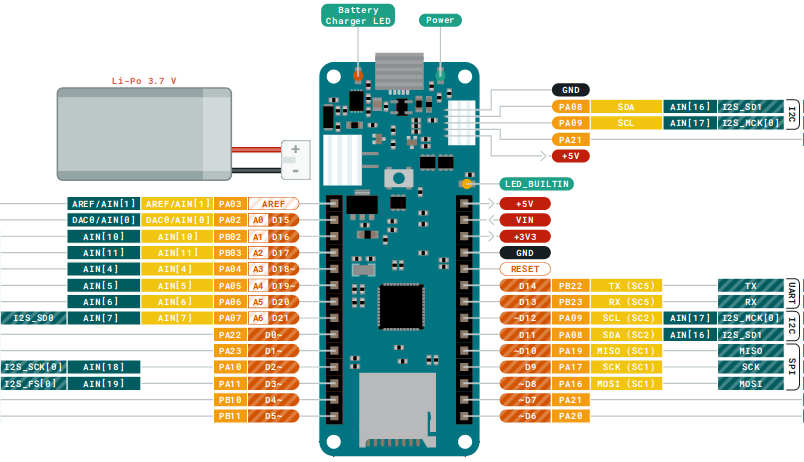
\includegraphics[width=0.9\textwidth]{MA/uM/uM}
    \caption{\mu M - pin out \cite{noauthor_arduino_2016-1}}
\end{figure}
\begin{table}[H]
    \centering
    \begin{threeparttable}[b]
        \begin{tabularx}{\linewidth}{ >
                    {\hsize=.25\hsize}X >
                    {\hsize=0.5\hsize}X >
                    {\hsize=.25\hsize}X  >
                    {\hsize=.5\hsize}X >
                    {\hsize=.25\hsize}X  >
                    {\hsize=3\hsize}X
            }
                  & \multicolumn{4}{c}{Pin mapping} &                                                                                                                   \\
            \cmidrule(lr){3-6}
            Id    & Net                             & Nb. & Name           & Type                           & Function                                                  \\
            \midrule
            $U_1$ & .Prx                            & 2   & \texttt{A0}    & \leftsquigarrow                & A/D conversion of OS output voltage                       \\
            $U_1$ & ESS                             & 9   & \texttt{D0}    & \rightharpoonup                & enable SS                                                 \\
            $U_1$ & ACK'                            & 10  & \texttt{D1}    & \leftharpoonup                 & .ACK connected via BI\textsubscript{1}                    \\
            $U_1$ & EOD                             & 11  & \texttt{D2}    & \rightharpoonup                & enable OD                                                 \\
            $U_1$ & EWD                             & 12  & \texttt{D3}    & \rightharpoonup                & enable WD                                                 \\
            $U_1$ & RWD                             & 13  & \texttt{D4}    & \rightharpoonup                & reset WD timer                                            \\
            $U_1$ & \neg .PB\tsc{1}                 & 14  & \texttt{D5}    & \leftharpoonup \upharpoonright & user push button                                          \\
            $U_1$ & .B'                             & 16  & \texttt{A1}    & \leftsquigarrow                & A/D conversion of scaled down battery voltage ( < 3.3 V)  \\
            $U_1$ & .S\textsubscript{1'c}           & 17  & \texttt{A2}    & \leftsquigarrow                & A/D conversion of scaled down solar voltage ( < 3.3 V)    \\
            $U_1$ & .S\textsubscript{2'c}           & 18  & \texttt{A3}    & \leftsquigarrow                & A/D conversion of scaled down solar voltage ( < 3.3 V)    \\
            $U_1$ & .SDA                            & 20  & \texttt{SDA}   & \leftrightharpoons             & .SDA connected via BI\textsubscript{2}                    \\
            $U_1$ & .SCL                            & 21  & \texttt{SCL}   & \leftrightharpoons             & .SCL connected via BI\textsubscript{2}                    \\
            $U_1$ & \neg RS                         & 24  & \texttt{RESET} & \leftharpoonup                 & pulled down by WD timer or user button in case of timeout \\
            $U_1$ & \Gnd                            & 25  & \texttt{GND}   & \Gnd                           &                                                           \\
            $U_1$ & 3V3                             & 26  & \texttt{VCC}   & $\rightarrow$                  & regulated output voltage\tnote{1}                         \\
            $U_1$ & .V\textsubscript{\mu M}         & 27  & \texttt{VIN}   & $\leftarrow$                   & unregulated input voltage >  \SI{3.5}{\V} \tnote{2}       \\
        \end{tabularx}
        \begin{tablenotes}
            \item [1] \begin{displayquote}[]\textelp{} This pin outputs 3.3V through the on-board voltage regulator.
                This voltage is the same regardless the power source
                used (USB, Vin and Battery) (\cite{noauthor_arduino_2016-1}).\end{displayquote}
            \item [2]  \begin{displayquote}[]\textelp{} This pin can be used to power the board with a regulated 5V source.
                If the power is fed through this pin, the USB power source is disconnected.
                This is the only way you can supply \SI{5}{V} (range is 5V to maximum 6V) to the board not using USB.
                (\cite{noauthor_arduino_2016-1}).             \end{displayquote}
        \end{tablenotes}
    \end{threeparttable}
\end{table}
\clearpage



\subsection{Bus Isolation Module (BI)}

The Bus Isolation Module (BI) allows the slave to interconnect its GPIO pins with equivalent pins of the \mu M module.
These pins are not designed to support voltages > 0 when the microcontroller is powered off.
Since the slave microcontroller
is powered on only during the transmission phase, the pins configured for I2C would effectively be back-powered via
the internal ESD protection diodes.

\subsubsection*{Specification}

The switch must have the following characteristics:
\begin{itemize}
    \item low power: this excludes mechanical switches like reed relays
    \item bidirectional
    \item 3.3V logic compatible
\end{itemize}

\subsubsection*{Implementation}

\begin{table}[H]
    \centering
    \begin{threeparttable}[b]
        \begin{tabularx}{\linewidth}{ >
                    {\hsize=0.25\hsize}X >
                    {\hsize=0.75\hsize}X >
                    {\hsize=1.25\hsize}X >
                    {\hsize=0.75\hsize}X >
                    {\hsize=2.0\hsize}X
            }
            Id    & BOM item                       & Order Code      & FF       & Rationale \\
            \midrule
            $U_1$ & \cite{noauthor_ts5a23157_2004} & TPD3S014-Q1/176 & VSSOP/10 & low Ron   \\
        \end{tabularx}
    \end{threeparttable}
    \caption{BI - BOM}
\end{table}




\begin{table}[H]
    \centering
    \begin{threeparttable}[b]
        \begin{tabularx}{\linewidth}{ >{\hsize=.15\hsize}X >{\hsize=1.35\hsize}X >{\hsize=1.5\hsize}X }
            Id & Issue                                       & Potential solutions \\
            \midrule
            1  & $U_{1,2}$ can not be back-powered.\tnote{1} & TMUX1574RSVR (TI)   \\
        \end{tabularx}
        \begin{tablenotes}
            \item [1]   Usually, the slave is not powered on when the master is powered off because
            the load switch for the slave power supply requires a logic H from the master to be on.
            However, when flashing (programming) the slave, the master could be switched off and in this
            case the supply voltage of $U_{1,2}$ if \SI{0}{\volt}.
        \end{tablenotes}
    \end{threeparttable}
    \caption{\mu M - Issues}

\end{table}
\clearpage


\begin{figure}[h]
    \centering
    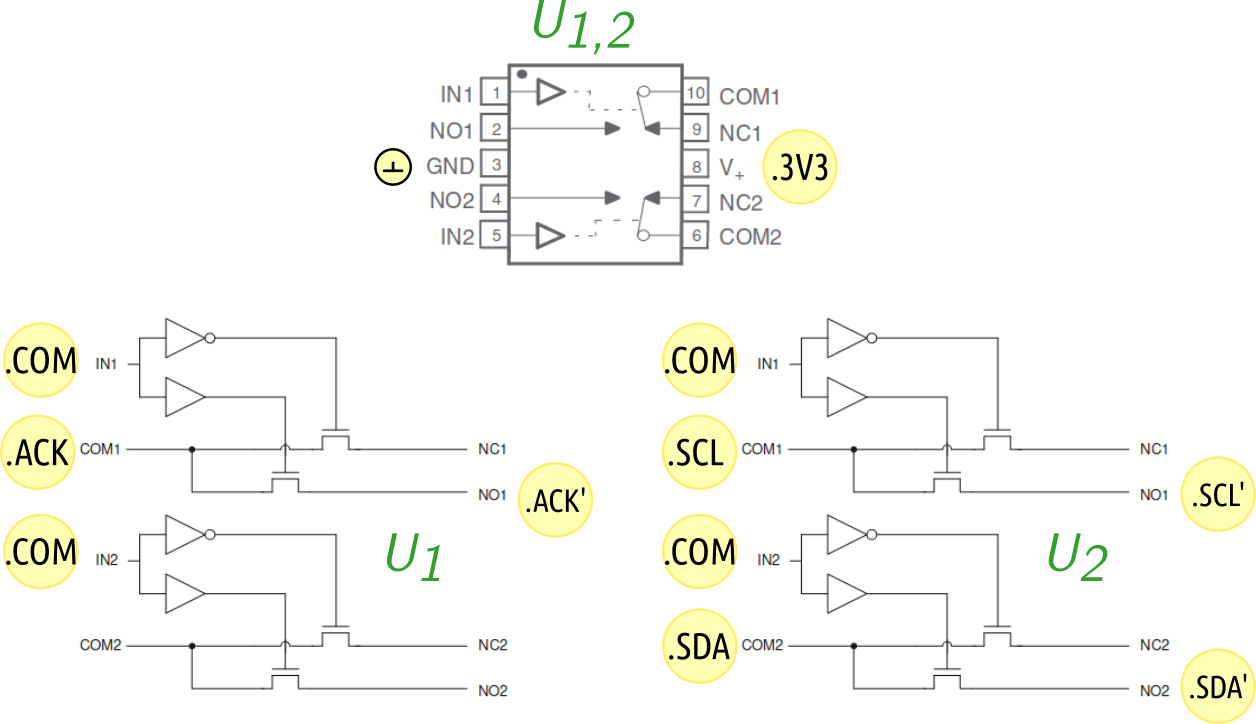
\includegraphics[width=1.0\textwidth]{MA/BI/BI}
    \caption{BI - schematic, based on datasheet \cite{noauthor_ts5a23157_2004}}
\end{figure}

\begin{table}[H]
    \centering
    \begin{threeparttable}[b]
        \begin{tabularx}{\linewidth}{ >
                    {\hsize=.25\hsize}X >
                    {\hsize=0.5\hsize}X >
                    {\hsize=.25\hsize}X  >
                    {\hsize=.5\hsize}X >
                    {\hsize=.25\hsize}X  >
                    {\hsize=3\hsize}X
            }
                  & \multicolumn{4}{c}{Pin mapping} &                                                                            \\
            \cmidrule(lr){3-6}
            Id    & Net                             & Nb. & Name          & Type            & Function                           \\
            \midrule
            $U_1$ & .COM                            & 1   & \texttt{IN1}  & \leftharpoonup  & switch 1 enable, driven by \mu S   \\
            $U_1$ & .ACK'                           & 2   & \texttt{NO1}  & \rightharpoonup & normally open, switch 1 output     \\
            $U_1$ & \Gnd                            & 3   & \texttt{GND}  & \Gnd            & \Gnd                               \\
            $U_1$ & .COM                            & 5   & \texttt{IN2}  & \leftharpoonup  & switch 2 enable, switch 2 not used \\
            $U_1$ & .3V3                            & 8   & \texttt{V+}   & \leftarrow      & power supply                       \\
            $U_1$ & .ACK                            & 10  & \texttt{COM1} & \leftharpoonup  & switch 1 input                     \\
            $U_2$ & .COM                            & 1   & \texttt{IN1}  & \leftharpoonup  & switch 1 enable, driven by \mu S   \\
            $U_2$ & .SCL'                           & 2   & \texttt{NO1}  & \rightharpoonup & normally open, switch 1 output     \\
            $U_2$ & \Gnd                            & 3   & \texttt{GND}  & \Gnd            & \Gnd                               \\
            $U_2$ & .SDA'                           & 4   & \texttt{NO2}  & \rightharpoonup & \Gnd                               \\
            $U_2$ & .COM                            & 5   & \texttt{IN2}  & \leftharpoonup  & switch 2 enable, switch 2 not used \\
            $U_2$ & .SDA                            & 6   & \texttt{COM2} & \leftharpoonup  & switch 2 enable, switch 2 not used \\
            $U_2$ & .3V3                            & 8   & \texttt{V+}   & \leftarrow      & power supply                       \\
            $U_2$ & .SCL                            & 10  & \texttt{COM1} & \leftharpoonup  & switch 1 input                     \\
        \end{tabularx}
        \begin{tablenotes}
            \item []
        \end{tablenotes}
    \end{threeparttable}

\end{table}
\clearpage



\subsection{Opto Switch Driver Module (OD)}

The Opto Switch Driver Module (OD) is an interface between module \mu M and the Opto Switch Module (OS).

\subsubsection*{Requirements}

Experiments have shown that at least \SI{50}{\mA} are required to obtain  clearly separated
voltage levels at the output of OS (.Prx).

\subsubsection*{Implementation}


\begin{figure}[h]
    \centering
    \includegraphics[width=0.8\textwidth]{MA/OD/OD}
    \caption{OD - schematic, based on datasheet \cite{noauthor_sn74lvc2g17_2002}}
\end{figure}

\begin{table}[H]
    \centering
    \begin{threeparttable}[b]
        \begin{tabularx}{\linewidth}{ >
                    {\hsize=.25\hsize}X >
                    {\hsize=0.5\hsize}X >
                    {\hsize=.25\hsize}X  >
                    {\hsize=.5\hsize}X >
                    {\hsize=.25\hsize}X  >
                    {\hsize=3\hsize}X
            }
                  & \multicolumn{4}{c}{Pin mapping} &                                                                             \\
            \cmidrule(lr){3-6}
            Id    & Net                             & Nb. & Name         & Type            & Function                             \\
            \midrule
            $U_1$ & .EOD                            & 1   & \texttt{1A}  & \leftharpoonup  & buffer input controlled by \mu C     \\
            $U_1$ & .EOD                            & 3   & \texttt{2A}  & \leftharpoonup  & buffer input controlled by \mu C     \\
            $U_1$ & \Gnd                            & 2   & \texttt{GND} & \Gnd            &                                      \\
            $U_1$ & Y                               & 4   & \texttt{1Y}  & \rightharpoonup & buffer output                        \\
            $U_1$ & .3V3                            & 5   & \texttt{VCC} & \leftarrow      & power supply                         \\
            $U_1$ & Y                               & 6   & \texttt{2Y}  & \rightharpoonup & buffer output                        \\
            $R_c$ & Y                               & 1   & \texttt{1}   &                 &                                      \\
            $R_c$ & .V\textsubscript{OS}            & 2   & \texttt{2}   &                 & anode voltage of photodiode          \\
            $R_p$ & .3V3                            & 1   & \texttt{1}   &                 & upper rail for pullup resistor       \\
            $R_p$ & .Prx                            & 2   & \texttt{2}   &                 & collector voltage of phototransistor \\
        \end{tabularx}
        \begin{tablenotes}
            \item []
        \end{tablenotes}
    \end{threeparttable}

\end{table}
\begin{table}[H]
    \centering
    \begin{threeparttable}[b]
        \begin{tabularx}{\linewidth}{ >{\hsize=.15\hsize}X >{\hsize=1.35\hsize}X >{\hsize=1.5\hsize}X }

            Id & Issue             & Potential solution      \\
            \midrule
            1  & power consumption & current source\tnote{1} \\
        \end{tabularx}
        \begin{tablenotes}
            \item [1] The current implementation is not ideal. It would be better to use a (programmable) current source to avoid burning power in the current
            limiting resistor. In addition, the optimum output current remains to be determined.
        \end{tablenotes}
    \end{threeparttable}
    \caption{OD - issues}
\end{table}
\clearpage
\begin{table}[H]
    \centering
    \begin{threeparttable}[b]
        \begin{tabularx}{\linewidth}{ >{\hsize=0.25\hsize}X >{\hsize=0.75\hsize}X >{\hsize=1.25\hsize}X >{\hsize=0.5\hsize}X >{\hsize=2.25\hsize}X}

            Id    & Desc                             & Order Code          & FF     & Rationale                                   \\
            \midrule
            $U_1$ & \cite{noauthor_sn74lvc2g17_2002} & SN74LVC2G17DCKR/473 & SC70/6 & high output power, parallel output\tnote{1} \\
            $R_p$ & \SI{1}{\kilo\ohm}                & generic             & 0603   & pull-up resistor\tnote{2}                   \\
            $R_c$ & \SI{20}{\ohm}                    & generic             & 0603   & current limit resistor \tnote{3}            \\
            $C_b$ & \SI{100}{\nF}, \SI{16}{\V}       & generic             & 0402   & bypass cap                                  \\
        \end{tabularx}
        \begin{tablenotes}
            \item [1] for a total rated maximum of \SI{48}{\milli\ampere}, low power consumption,
            the Smitt-Trigger inputs are not really necessary for this application.
            \item [2] We should explain why we choose this value. But as mentioned in Issue 1, we are likely
            to replace the current limit resistor with a current source in the near future.
            \item [3] idem
        \end{tablenotes}
    \end{threeparttable}
    \caption{OD - BOM}
    \label{table:wd1}
\end{table}















